\documentclass{standalone}
\usepackage{preset}
\begin{document}
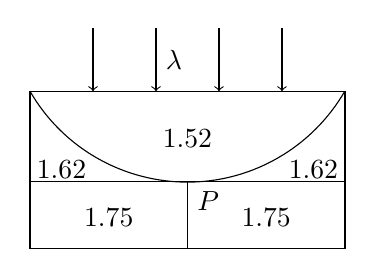
\begin{tikzpicture}[x=20mm,y=20mm]
	\draw(0,0)rectangle+(2,1);
	\draw(0,0)rectangle+(1,.424);
	\draw(1,0)rectangle+(1,.424);
	\draw(0,1)arc(-150:-30:1.154);
	\draw[->](.4,1.4)--+(0,-.4);
	\draw[->](.8,1.4)--node[right]{$\lambda$}+(0,-.4);
	\draw[->](1.2,1.4)--+(0,-.4);
	\draw[->](1.6,1.4)--+(0,-.4);
	\draw(1,.7)node{1.52};
	\draw(.2,.5)node{1.62};
	\draw(1.8,.5)node{1.62};
	\draw(.5,.2)node{1.75};
	\draw(1.5,.2)node{1.75};
	\draw(1,.424)node[below right]{$P$};
\end{tikzpicture}
\end{document}
